%----------Latex-------------
% contain a description of Kurans model


\subsection{Kuran's Unanticipated Revolutions} 
\label{sec:Kuran}

Most of the well known revolutions like the French revolution of 1789, the Russian Revolution of February 1917 and the Eastern bloc revolution of 1989, evolved surprisingly fast. The most recent example is the Arabian Spring. The economist Timur Kuran developed a model to explain why the suppression of the government works fine for a long period and then a revolution can grow entirely unexpected in a very short time span. \cite{Kuran_1989}
To explain that phenomena, Kuran described a expressive equilibrium in which the opposition is forced to remain hidden and is strongly discouraged out of fear from the government. But as soon as a few individuals speak up, they can eventually spark a revolution, because now other individuals dare to express their opinion as well.
Like most economists Kuran assumes, that the individuals act rational. Furthermore he assumes, that every individual has two opinions. One is the actual private opinion, the private preference and the other is the publicly expressed opinion, the public preference, that is shown to the other members of the society. The case in which an individual's public and private preference don't match is referred to as preference falsification. While the private actual opinion changes slowly over a longer time period, the publicly expressed opinion can change rather fast, since it is only the decision of the individual to lie or not to lie about his actual opinion. 
To decide whether or not to change the publicly expressed opinion, the individual has to way of his the (expected) costs of punishment in case of a failure of the revolution and the cost of preference falsification. The point at which the costs match each other is the individual's threshold.  Because Kuran assumes that the expected costs of opposition depend on the size of the opposition movement, the threshold depends on the actual opinion and the size of the opposition. Dependent on the threshold contribution, a revolution can cascade reasonably fast. \cite{Donnay_2011}
To Illustrate how the revolution can develop in theory lets take a stair like distribution of the thresholds as shown in figure \ref{casecadethreshold} with 10\% of the individuals with a threshold of 0, 10\% with a threshold of 0.1, 10\% with a threshold of 0.2 and so on. The first 10\% will start the opposition immediately, but then the threshold of the second 10\% is reached and the change of the public preference cascades through the whole population.
\begin{figure}[!b]
\centering
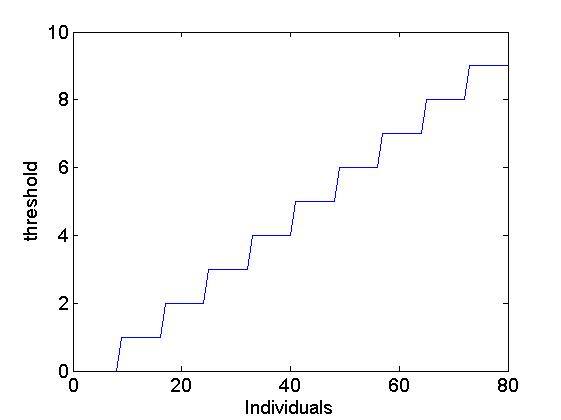
\includegraphics[width=0.55\textwidth, keepaspectratio=true]{cascadethresholddistripution.jpg}
\caption{stair like distribution of the thresholds}
\label{cascadethreshold}
\end{figure}
